

\documentclass{article}
\usepackage[utf8]{inputenc}
\usepackage[english]{babel}
\usepackage{authblk}
\usepackage{setspace}
\usepackage[margin=1.25in]{geometry}
\usepackage{graphicx}
\graphicspath{ {./figures/} }
\usepackage{subcaption}
\usepackage{amsmath}
\usepackage{biblatex}
\addbibresource{sample.bib}


%%%%%% Bibliography %%%%%%
% Replace "sample" in the \addbibresource line below with the name of your .bib file.

%%%%%% Title %%%%%%
% Full titles can be a maximum of 200 characters, including spaces. 
% Title Format: Use title case, capitalizing the first letter of each word, except for certain small words, such as articles and short prepositions
\title{Multi Threaded Java Sorting Library}

%%%%%% Authors %%%%%%
% Authors should be listed in order of contribution to the paper, by first name, then middle initial (if any), followed by last name.
% Authors should be listed in the order in which they will appear in the published version if the manuscript is accepted. 
% Use an asterisk (*) to identify the corresponding author, and be sure to include that person’s e-mail address. Use symbols (in this order: †, ‡, §, ||, ¶, #, ††, ‡‡, etc.) for author notes, such as present addresses, “These authors contributed equally to this work” notations, and similar information.
% You can include group authors, but please include a list of the actual authors (the group members) in the Supplementary Materials.


\author{
  Kenneth Bicknell, Michael Ortiz, William Presswood, Mike Triana, and \newline Stefan Werleman\\
}

%%%%%% Spacing %%%%%%
% Use paragraph spacing of 1.5 or 2 (for double spacing, use command \doublespacing)
\onehalfspacing

\begin{document}

\maketitle

%%%%%% Abstract %%%%%%
\begin{abstract}
%The abstract should be a single paragraph written in plain language that a general reader can understand. Do not include citations, figures, tables, or undefined abbreviations in the abstract. Any abbreviations that appear in the title should be defined in the abstract. The length should be 200 words and not exceed 300 words, to include: 
%\begin{itemize}
%    \item An opening sentence that states the question/problem addressed by the research AND
%    \item Enough background content to give context to the study AND
%    \item A brief statement of primary results AND
%    \item A short concluding sentence.
%\end{itemize}

With the rise of e-commerce and the digital age, companies have an abundance of data that they need to make sense out of. Internet speeds are also ever increasing, which now means that the main bottle neck of a system could be the server that is running the algorithms. We are also seeing diminishing returns on Moore's law, which means that you can no longer count on the newest processor being enough for your needs. With data centers and even in home computing, our computers are becoming more parallel, so we decided to find ways to make the most known algorithms concurrent. The results indicate that divide and conquer is still the way to go.
\end{abstract}

%%%%%% Main Text %%%%%%

\section{Introduction}

% Explain problem
Modern computer systems frequently transmit, store, and manipulate large amounts of data. To make this data easier to manage, it is desirable to have the ability to sort it. Sorted collections of data are often much more convenient to work with. Looking up a word in an alphabetically sorted dictionary is a far easier task than finding a word in a randomly shuffled set of cards. Although programs can run more efficiently with sorted data, sorting the data in the first place takes time and effort, especially for significantly large collections. If our sorting algorithm is too slow, it defeats the purpose of improving program efficiency. We therefore desire sorting algorithms that are relatively fast for large inputs.

% Justify research
A variety of approaches to developing fast sorting algorithms have arisen, though many of them still fail to perform well on large data sets. One way to improve performance for many programs is to use multiple threads to divide the work into multiple processes that can be executed concurrently. Several sorting techniques which are often implemented as sequential algorithms possess qualities that suggest they may benefit from using concurrency.

Of course, introducing multiple threads presents its own problems with respect to speed and efficiency. Special precautions must be taken to ensure that work performed by concurrently running threads remains valid, and these precautions can delay progress during execution. This presents the question: Can sorting algorithms be made more efficient by using multiple threads? If so, which ones, and by how much?

% Explain goals of research
The goal of this project is to improve the efficiency of several common sorting algorithms by redesigning them to use multiple threads. We have chosen to focus on the following algorithms due to their popularity and their potential, we believe, to demonstrate significant improvement as parallel versions:
\begin{itemize}
  \item Bubble sort
  \item Bucket sort
  \item Insertion sort
  \item Merge sort
  \item Quick sort
  \item Selection sort
\end{itemize}
We will discuss our approaches to designing parallel versions of each sorting algorithm. Once we obtain a working parallel implementation of each algorithm, we will perform empirical run-time analysis to compare their performance to their sequential counterparts. We will then discuss the implications of these results and the practicality of our implementations.

\section{Materials and Methods}
\subsection{Java}
For this project, we will be writing sequential and concurrent implementations of sorting algorithms in the Java programming language. Java was chosen mainly due to the team's experience with the language, as well as its convenient packages for managing threads.

\subsection{Java's Concurrent Package}
Java's Thread, Executor, ReentrantLock, and ExecutorService libraries will mostly be used to implement all algorithms concurrently. \cite{javathread, javalibs, javalock, executor} 

\subsection{Online Resources}
To allow us to focus on developing parallel versions of the algorithms, we chose to borrow sequential implementations from other authors, including Baeldung.com, GeeksforGeeks.org and InterviewDojo.com.

\subsection{Data Analysis}
\begin{itemize}
  \item Python's Pandas was used to record empirical run-time analysis results
  \item Python's MatPlotLib was used to produce all of graphs and charts.
\end{itemize}

% Describe sequential designs of each algorithm
\section{Sorting Algorithms: Sequential}
In the following section, we will briefly discuss the traditional sequential design of each sorting algorithm and analyze its efficiency in terms of time complexity.

\subsection{Bubble Sort}
Bubble sort is an algorithm that traverses an array $n-1$ times, $n$ being the number of elements in the array, giving it a Big O of O($n^2$). Each time the array is traveled it compares adjacent elements to find out which is greater or lesser, depending on the desired array outcome. With each comparison elements will move up or down the array until the traversal reaches the $n-i$th position, where $i$ is the number of iterations, and the greatest or least element in that iteration “bubbles” to the top.\cite{bubbleSort}

\subsection{Bucket Sort}
Bucket sort, also known as bucket sort, is an algorithm that caches the frequency of all the values in the array into to a frequency array. The process begins with traversing through the list and each element you access will be an index of the frequency array, also known as the bucket. For every index you access in the bucket, you increment value by one. This step repeats itself until then end of the list. The final step is to traverse through the bucket with each element containing a value called it's frequency. If the frequency is greater than zero, than you insert the element into the original list until the frequency is zero. After the bucket traversal, the original will now be sorted.

\subsection{Insertion Sort}
Insertion sort works well for small lists. It works by splitting the list into a sorted and unsorted section. Initially the sorted part is just the first element of the list and the unsorted part is the rest. Insertion sort iterates over every element in the unsorted list and places it in the correct place within the sorted list. Insertion sort has an average and worst case run time of O($n^2$).
\subsection{Merge Sort}
Merge sort is one of the most fundamental sorts in every computer science program. It takes advantage of one of the core concepts we use as CS students, divide and conquer. We take the original array and break it up into the smallest pieces we can by breaking it in half and then take n time to sort those two sorted halves back into one This gives the algorithm a run time of O($n*log(n)$) $n$ time to sort each sub array and $log(n)$ time to break the original down into the sub arrays.\cite{mergeSort}
\subsection{Quick Sort}
Quick sort is a lot like merge sort in the sense that it uses divide and conquer. It takes a certain partition in the array and makes sure that all data in the array that comes before it comes before the partition elements and all data that is larger comes after the partition. You achieve this by swapping smaller values at the start of the list with larger elements after in O($n$) time. You then break the array into two smaller sub arrays and perform the same on each half. Going through each half take O($n$) time and it happens $log(n)$ times so the total run time is O($n*log(n)$)
\subsection{Selection Sort}
Like insertion sort, selection sort divides the list into a (initially empty) sorted section on the left side and an unsorted section on the right side. The algorithm finds the smallest value in the current unsorted section of the list and moves it to the end of the sorted section. This is done by swapping said element with the leftmost unsorted element and expanding the boundaries of the sorted section so it includes the repositioned element. This process continues until the sorted section encompasses the entire list. The algorithm performs $n-1$ steps, scanning $n-i$ elements on the $i$th step. This results in an average complexity of O($n^2$).

% Describe hypotheses for parallel designs of each algorithm
\section{Sorting Algorithms: Parallel}
In the following section, we will discuss our approaches to designing parallel versions of each sorting algorithm and analyze their complexity in relation to their sequential counterparts.

\subsection{Bubble Sort}
To parallelize bubble sort, the best outcome currently is simple but should yield decent increase of speed. The method will take an unsorted array and make a duplicate of it, with each array assigned to a single thread. The first thread will be using bubble sort from the first element and work its way to the last element bringing the heaviest weights to the back for length/2 times, while the second thread takes the first element and traverses to the last element in the array taking the lightest weights to the back for length-midpoint times, can be reversed depending on desired result from sorting. Since we are dividing this task up into two parts, the first thread will iterate $n/2$ times, while the second will iterate $n-n/2$ times. When both threads complete, their arrays will be merged into a third array, where array 2 is the first half of the array, which the program will traverse from the second array's end to the length-midpoint-1, adding each value to the final array from index 0 on. The first array will start at the midpoint and work its way to the end adding values to the third array from length-midpoint to the last index. Theoretically this could cut the time of bubble sort in half.

\subsection{Bucket Sort}
Given that the run-time for bucket sort is: \[ O(n + m) \] With n being the length of the input array and m being the length of the bucket. There is one major functions that iterate through the input array. and the loop that caches all of the values in the array.

To parallelize the algorithm, the program partitions the array amongst the total number of threads the local machine has. The total number of threads is denoted as: \[T\] If n is less than or equal to T, the program will spawn n threads and assign each thread to an element in the array to run the caching process. Otherwise, the program will spawn T threads and split the work amongst all threads, T. This should have a speed-up on the O(n) execution part of the overall run-time. To verify the speed, empirical run-time analysis will be done.

\subsection{Insertion Sort}
It is tricky to imagine an easy way to parallelize an algorithm such as insertion sort since it is sequential in nature. One potential way is to capitalize on the structure of merge sort, which as divide and conquer algorithm, more naturally lends itself to multi-threading. So, partition the list into $n$ parts (given $n$ threads) and have each thread independently perform the standard sequential insertion sort on its section of the list. Finally, after all threads have completed, have the main thread perform a merge operation and yield the final sorted array. This approach should theoretically yield faster results than the sequential version on large inputs, but empirical run time analysis is needed to verify. This approach can also be applied to an optimisation on insertion sort known as shell sort. Shell sort works by partitioning the input list based on an ever shrinking gap value and independently sorting these sub lists. This is repeated until the gap value is 1, at which point a normal insertion sort is performed on an almost sorted list. Shell sort is much faster than normal insertion sort and is more inherently parallelizable, therefore we decided to develop our concurrent approach using the shell sort algorithm. 
\subsection{Merge Sort}
It is quite easy to imagine a way to make merge sort concurrent. The easiest way would be to just break up your original array in $n$ sub arrays based on the number of threads you have and then merge them back together after they are each sorted and re-merged. This is a bit of a naive way of performing merge sort and has to have hard coded number of threads and a hard coded joiner. This way really only works if you now a lot about the system you are running the program on and it has an average or less number of cores. There is no locks so the speed up should be pretty good for the effort put in.\newline
Another way to make merge sort concurrent would be to spin up a new thread every time you made a sub array. This would prevent you from having to manually break up the array and stitch it back together but the problem here is you would have to prevent the algorithm from spinning up crazy number of threads. If you were to spin up as many threads as you make sub arrays your system could come to a halt, with substantial enough $n$, from the overhead of all those threads. this means you would need to implement a minimum size where instead of starting a new thread you just sort the rest in the existing thread to avoid the bottle neck from lack of resources. this version of merge sort works well in conditions where you have lots of cores and lots of data. this way the overhead from cores does not completely out weigh the time it takes to just sort the data.
\subsection{Quick Sort}
Quick sort would use basically the same method as described in merge sort. You break the array up into smaller sub arrays and then perform quick sort on the smaller arrays. again this works in lower budget machines or in smaller data sets.\newline Or you could have the current thread partition the sub array and then break it up into two halves. You then give each of those 2 halves their own thread to to partition and break up their sub-arrays. You do encounter the same problem with thread overhead and need to seed a minimum size to avoid having millions of threads and bottle necking the whole system.
\subsection{Selection Sort}
Due to its similarities to insertion sort, we took a similar approach in regards to parallelizing selection sort. The list is partitioned into several sublists, which are sorted independently by individual threads. The resulting sorted sublists are then merged together to obtain the sorted list. To simplify the process of merging the sublists, we experimented with a different approach to divide the elements among the threads. Rather than partition the list based on index, the algorithm instead assigns each thread a range of values that cover a fraction of the total range of the list. Each thread sorts the elements in the list that fall within its range. Merging these sublists is trivial, as they can simply be joined end-to-end.

The complexity of this approach is slightly more difficult to analyze, as it now depends on the data contained in the list. Assuming the data is evenly distributed, it is divided among $m$ threads roughly evenly, tasking each thread with sorting $n/m$ elements. This results in an average complexity of O($(n/m)^2$). In the worst case, the data may be heavily skewed so that nearly all elements fall within the range assigned to a single thread. Such a case regresses back into sequential selection sort, giving the algorithm a worst-case complexity of O($n^2$).

\section{Results}
\subsection{Bubble Sort}
Unfortunately concurrent bubble sort was not as efficient when the hypothesised algorithm was implemented. The time comparison was at best case equal to sequential and worst case was around double the time. We feel that this was due to the traversal of multiple arrays to eventually have a single arrray that is sorted.
\subsection{Bucket Sort}
The concurrent version of bucket sort successfully sorts an array with a wide range of values. Unfortunately, it failed to significantly optimize the performance of the algorithm. There was very little speed-up between the sequential and parallel versions. This is probably due to the amount of overhead work that the Thread library requires.\newline
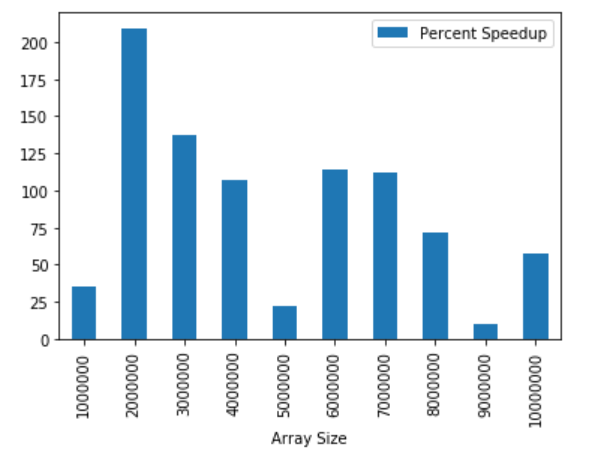
\includegraphics{figures/bucketbar.PNG}\newline
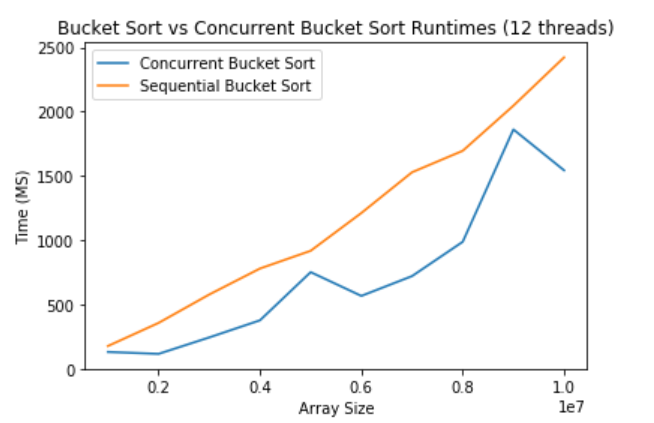
\includegraphics{figures/bucketline.PNG}
\subsection{Merge Sort}
Merge sort was one of our easiest to imagine sorts, and understandably so, with its emphasis on divide and conquer. We decided to use the approach where we divide the array into smaller arrays and then run merge sort on each of the smaller arrays. This method allows us to get the best performance with the least amount of fine tuning. With this approach, we are seeing a roughly 100\% speed up with 4 threads.\newline
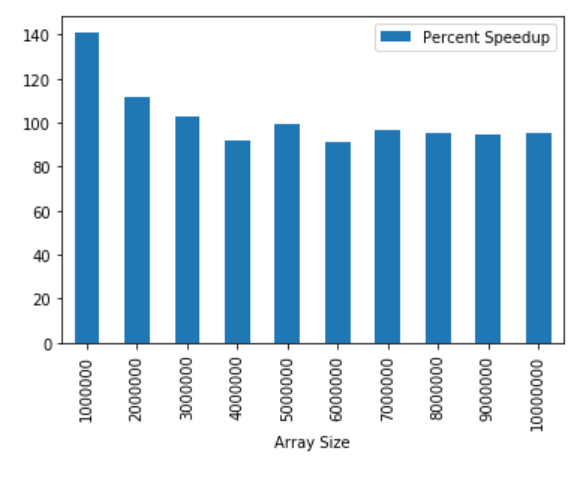
\includegraphics{figures/mergebar.PNG}\newline
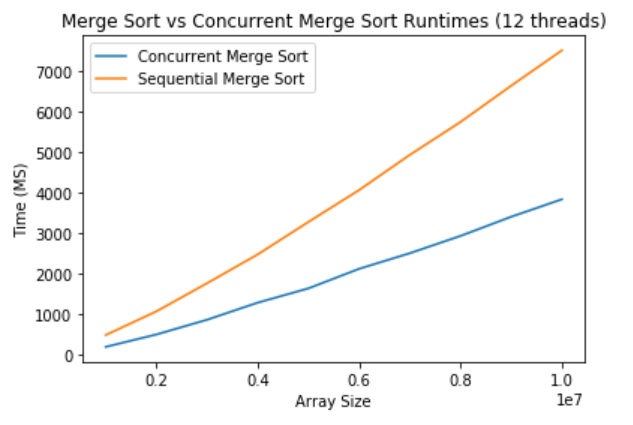
\includegraphics{figures/merge_line.PNG}
\subsection{Quick Sort}
Quick sort is also a divide and conquer algorithm. This makes it very easy to divide work between threads. In quick sort, we also used the approach where you divide the array into $n$ sub arrays and then perform quick sort on each of those. This allows us to tune the algorithm to our specific computers and avoid fine tuning of size limits. Unfortunately, this approach only netted about a 40\% speed up with 4 threads. This is likely due to how partitioning quickSort is not always an even split, and we can spend more time in one half of a split.
\newline
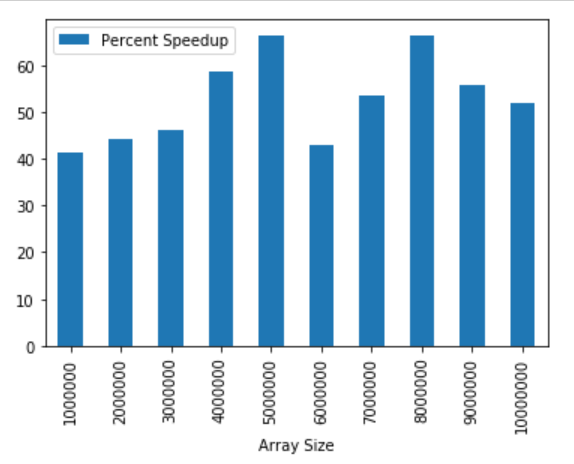
\includegraphics{figures/quickbar.PNG}\newline
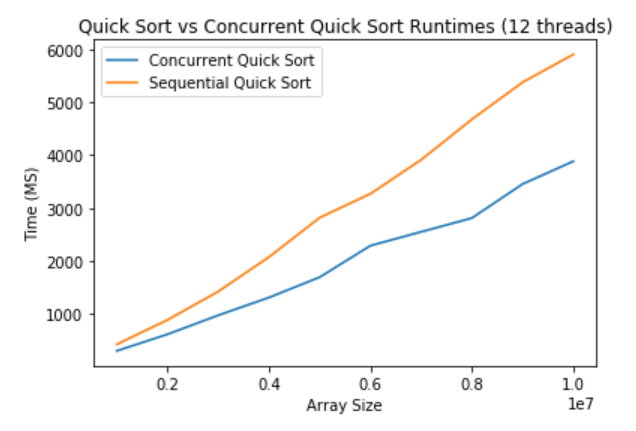
\includegraphics{figures/quickline.PNG}
\subsection{Shell Sort}
Shell sort is one of the sorts that really surprised us. We were original struggling to think of a way to make a concurrent version but as you can see in the graph when we ran it with  12 threads we had around a 400\% increase in speed. we were also able to make a version that scales well with different amounts of threads.\newline
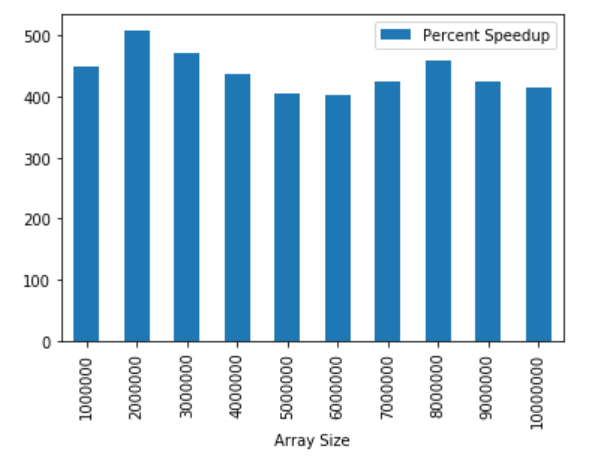
\includegraphics{figures/shellbar.PNG}\newline
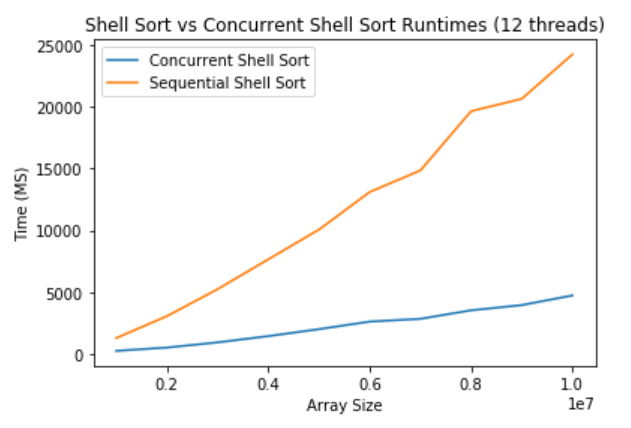
\includegraphics{figures/shellline.PNG}
\subsection{insertion Sort}
Selection Sort was the biggest surprise to us. Selection sort is one of the most intuitive sorts but is also one of the slowest that actually try to sort stuff. With our concurrent version we were amazed to see speed increases of up to 1400\%\newline
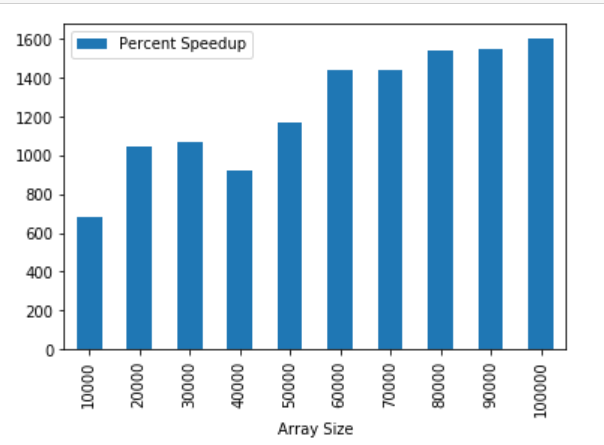
\includegraphics{figures/selectionbar.PNG}\newline
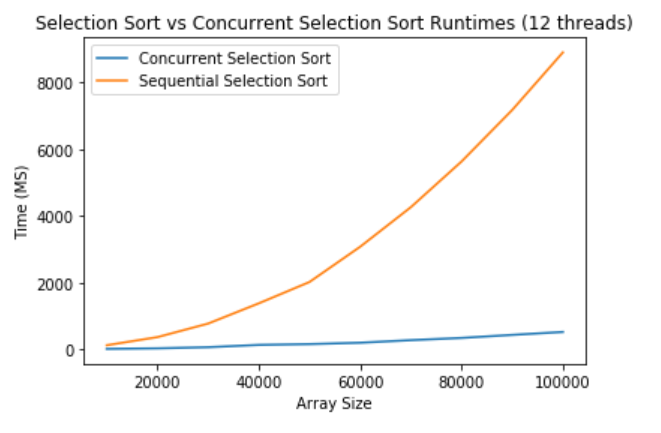
\includegraphics{figures/selectionline.PNG}

\section{Conclusion}
With our results it is clear to see that while it is difficult to implement concurrency has a great effect on the fundamental algorithms we learned in Computer Science 1. we were able to show great improvement in not only the divide and conquer algorithms but also in the algorithms that we typically consider slow. this makes it very worth it for companies to invest in multiple compute nodes and to invest in the development time to design for them.

\section{Appendix}
\subsection{Challenges}
\begin{itemize}
  \item Finding a meeting time that works for everyone
  \item Trying to design a super-type / interface for our sorting classes
  \item Making some algorithms are built with sequentialness in mind making them difficult to make concurrent
  \item Setting some of the container classes to be Generic in order to take in any datatype.
  \item Using some of Java's concurrent libraries\cite{javalibs} made it difficult for us to handle different types of exceptions.
\end{itemize}
\printbibliography{}

\end{document}